\chapter{Motif-Based Clustering} \label{chap:motif}

We analyse the performance of motif-based random-walk spectral clustering on both synthetic and real data.
In Section~\ref{sec:motif_dsbms} we propose a family of stochastic block models and perform experiments with a variety of motifs and parameters.
In Section~\ref{sec:motif_polblogs} we analyse the US Political Blogs network and in Section~\ref{sec:motif_migration} we present results from the US Migration network.






\section{Directed stochastic block models} \label{sec:motif_dsbms}

We begin by describing \emph{directed stochastic block models} (DSBMs), a broad class of generative models for directed graphs. A DSBM is characterised by a block count $k$, a list of block sizes $(n_i)_{i=1}^k$ and a sparsity matrix $F \in [0,1]^{k \times k}$. We define the cumulative block sizes $N_i = \sum_{j=1}^i n_j$ with $N_0=0$, and the total graph size $N=N_k$. These are used to construct the expected adjacency matrix $A \in [0,1]^{N \times N}$ given by $A_{ij} = F_{rs} \ \bb{I}\{i \neq j\}$ where $N_{r-1} < i \leq N_r$ and $N_{s-1} < j \leq N_s$. Finally a graph $\ca{G}$ is generated with adjacency matrix entries $G_{ij} \sim \textrm{Ber}(A_{ij})$ sampled independently. We say that a DSBM is \emph{symmetric} if $F$ is a symmetric matrix.

This DSBM definition is similar to that given by \cite{DirectedClustImbCuts}, although we impose independence between all entries of the adjacency matrix, allowing for bidirectional edges.


\subsection{Symmetric two-block DSBMs}


We define the \emph{symmetric two-block DSBM} as the DSBM with $k=2$, $n_1=n_2=n$ and $F = \begin{psmallmatrix} p & q \\ q & p \end{psmallmatrix}$ where $p > q$. Figure~\ref{fig:sym_two_block_dsbm} illustrates the block structure and sparsity matrix of this model. Thicker lines indicate existence of edges with higher probability.


\begin{figure}[H]
	\centering
	\includegraphics[scale=0.8,draft=false]{../tikz/sym_two_block_dsbm/sym_two_block_dsbm.pdf}
	\caption{Symmetric two-block DSBM block structure and sparsity matrix}
	\label{fig:sym_two_block_dsbm}
\end{figure}


We test the performance of Algorithm~\ref{alg:motifrwspectclust} across various motifs with parameters $k=l=2$ on this model.
Figure~\ref{fig:motifsym} shows violin plots over 20 trials of ARI against motif, for different sets of parameters $n,p,q$.
Also shown is $|C|$, the average size of the largest connected component of each MAM.
It can be seen that several motifs (such as $\ca{M}_5$ and $\ca{M}_9$) achieve a similar ARI to the traditional spectral clustering technique given by the symmetrised adjacency matrix $M=G+G^\top$ generated by the motif $\ca{M}_\mathrm{s}$ (Table~\ref{tab:motif_adj_mat_table}).
However the strongly connected motifs (particularly $\ca{M}_4$) generate MAMs with small connected components, especially when $\ca{G}$ is sparse, and hence only cluster a subset of the vertices of $\ca{G}$.

\begin{figure}[H]
	\begin{subfigure}{.49\textwidth}
		\centering
		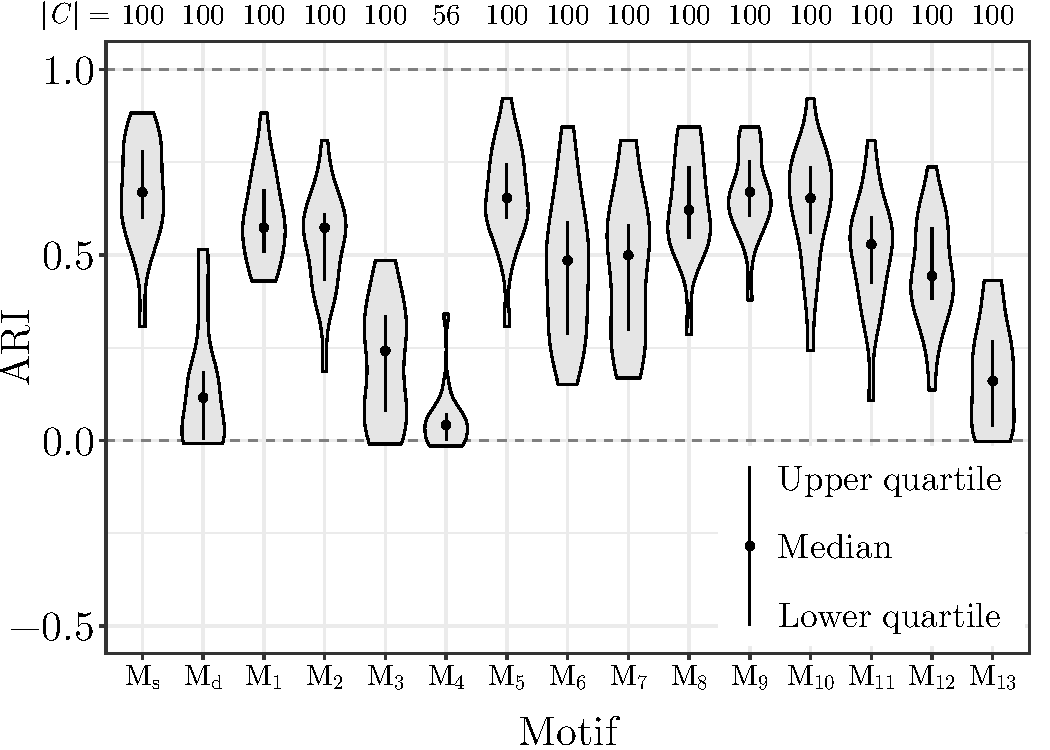
\includegraphics[scale=0.4,draft=false]{../../results/motifsym/motifsym_1.pdf}
		\caption{$n=50$, $p=0.3$, $q=0.2$}
	\end{subfigure}
	\begin{subfigure}{.49\textwidth}
		\centering
		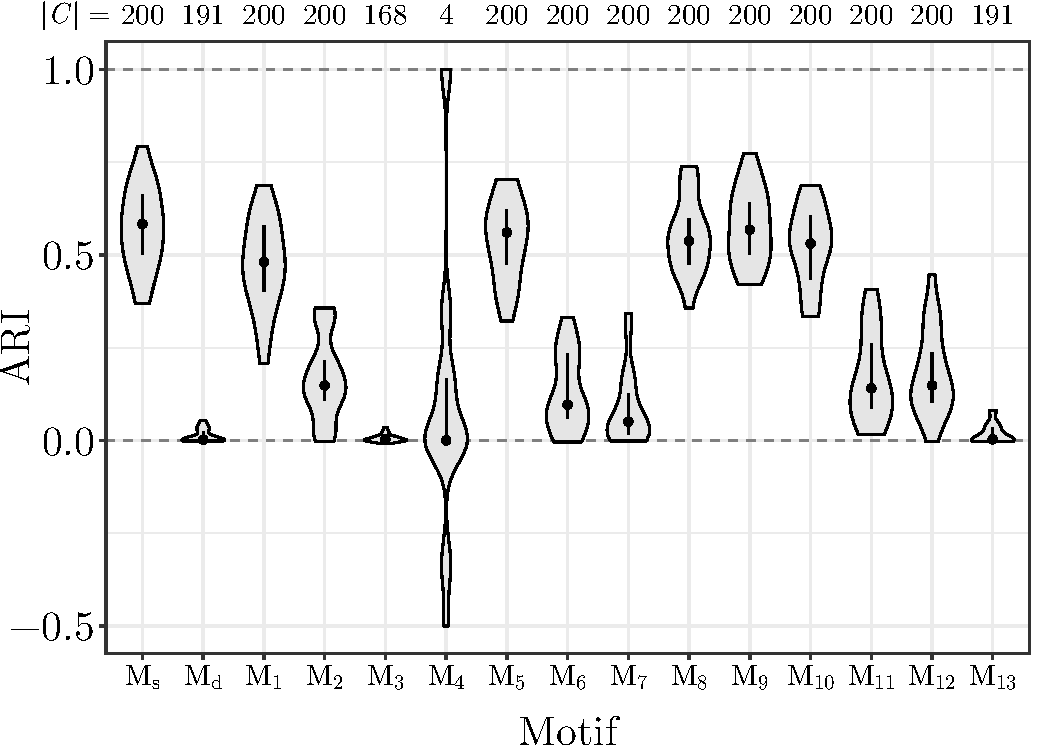
\includegraphics[scale=0.4,draft=false]{../../results/motifsym/motifsym_2.pdf}
		\caption{$n=100$, $p=0.15$, $q=0.1$}
	\end{subfigure}
	\caption{ARI violin plots for the symmetric two-block DSBM}
	\label{fig:motifsym}
\end{figure}






\subsection{Asymmetric two-block DSBMs} \label{sec:motif_asymm_dsbms}

We define the \emph{asymmetric two-block DSBM} as the DSBM with $k=2$, $n_1=n_2=n$ and $F = \begin{psmallmatrix} p & q_1 \\ q_2 & p \end{psmallmatrix}$ where $q_1 > q_2$ and $p = \frac{1}{2}(q_1+q_2)$. Figure~\ref{fig:asym_two_block_dsbm} shows this model.


\begin{figure}[H]
	\centering
	\includegraphics[scale=0.8,draft=false]{../tikz/asym_two_block_dsbm/asym_two_block_dsbm.pdf}
	\caption{Asymmetric two-block DSBM block structure and sparsity matrix}
	\label{fig:asym_two_block_dsbm}
\end{figure}

We test the performance of Algorithm~\ref{alg:motifrwspectclust} across various motifs with parameters $k=l=2$ on this model.
Figure~\ref{fig:motifasym} shows violin plots over 20 trials of ARI against motif, for different sets of parameters $n,p,q_1,q_2$, and $|C|$ is shown.
It is apparent that motif-based clustering with $\ca{M}_1$ is the best method, consistently achieving the highest ARI and keeping $|C|$ at its maximum value of $2n$.
It is unsurprising that $\ca{M}_1$ (feed-back loop) performs well on this model; large $p$ makes feed-back loops within clusters likely, and small $q_2$ makes feed-back loops spanning the clusters unlikely. Motif $\ca{M}_2$ also performs reasonably well since it contains $\ca{M}_1$ as a submotif.
Furthermore, the constraint $p = \frac{1}{2}(q_1+q_2)$ ensures that the na\"ive symmetrisation $M=G+G^\top$ produces indistinguishable clusters, and hence the traditional method performs extremely poorly.


\begin{figure}[H]
	\begin{subfigure}{.49\textwidth}
		\centering
		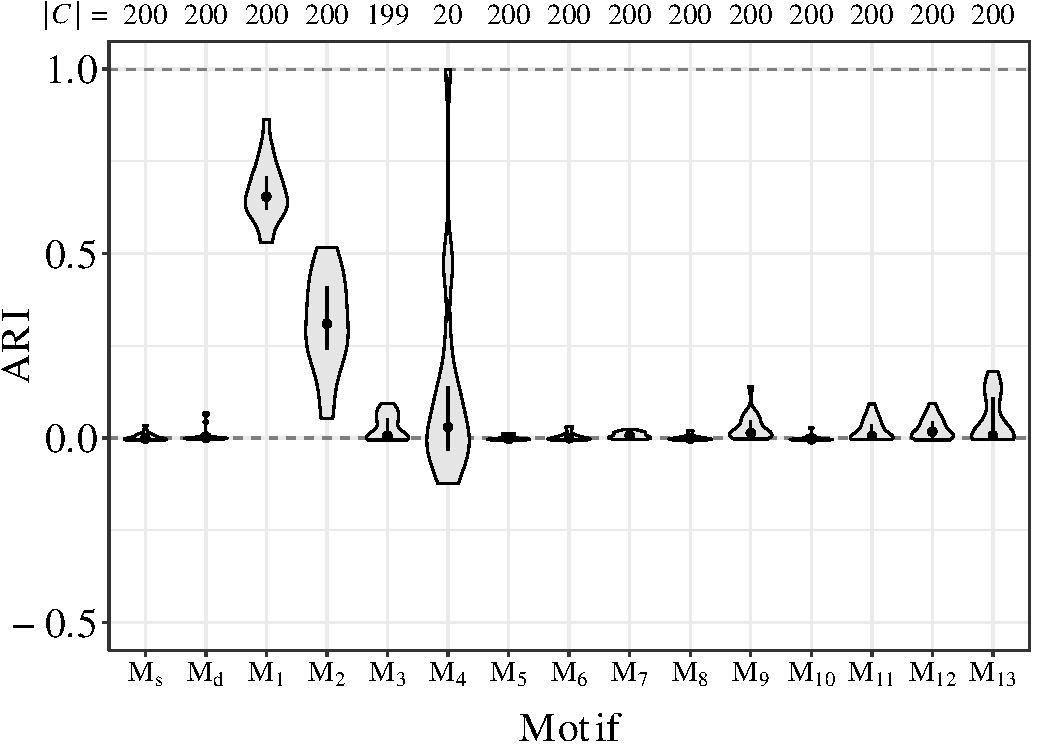
\includegraphics[scale=0.4,draft=false]{../../results/motifasym/motifasym_1.pdf}
		\caption{$n=100$, $p=0.2$, $q_1=0.35$, $q_2=0.05$}
	\end{subfigure}
	\begin{subfigure}{.49\textwidth}
		\centering
		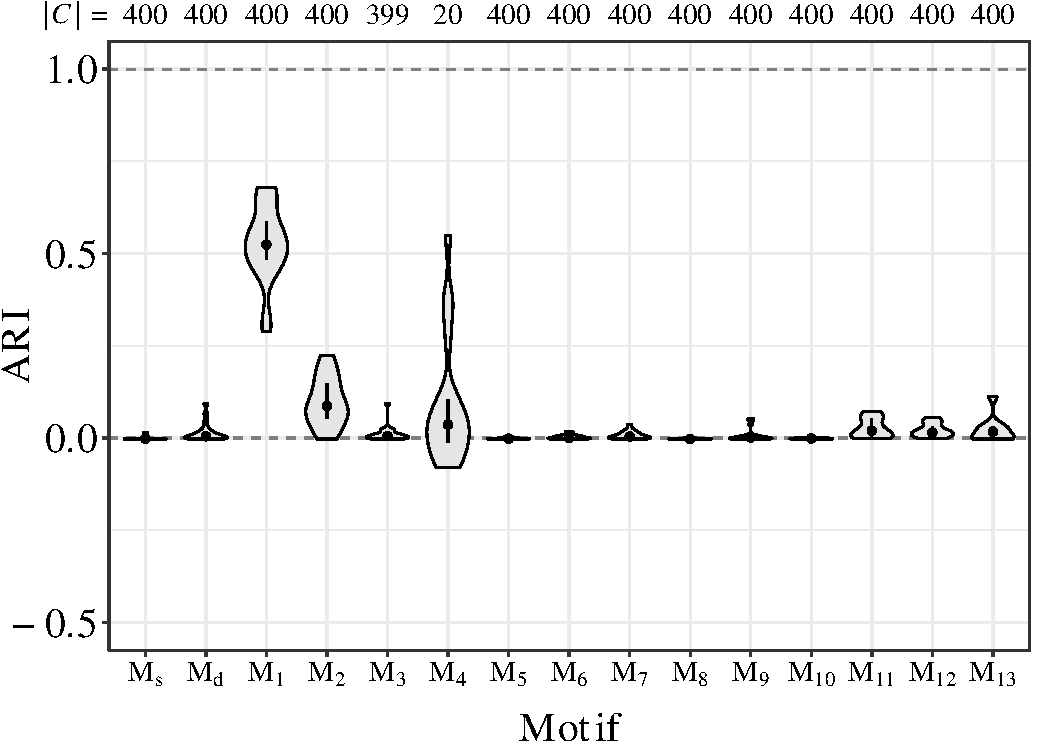
\includegraphics[scale=0.4,draft=false]{../../results/motifasym/motifasym_2.pdf}
		\caption{$n=200$, $p=0.15$, $q_1=0.25$, $q_2=0.05$}
	\end{subfigure}
	\caption{ARI violin plots for the asymmetric two-block DSBM}
	\label{fig:motifasym}
\end{figure}











\section{US Political Blogs network} \label{sec:motif_polblogs}

Our first real data set is the US Political Blogs network \cite{adamic2005political}, consisting of data collected two months before the 2004 US election. Vertices represent blogs, and are labelled by their political leaning (`liberal' or `conservative'). Weighted directed edges represent the number of citations from one blog to another. After preprocessing (Section~\ref{sec:notes_preprocessing}) there are $536$ liberal blogs, $636$ conservative blogs (total 1222) and $19 \, 024$ edges. The network is plotted in Figure~\ref{fig:polblogs_network}.

We test the performance of Algorithm~\ref{alg:motifrwspectclust} across various motifs with parameters $k=l=2$ on this network.
Figure~\ref{fig:polblogs_ariplot} plots ARI against component size $|C|$.
There is an apparent trade-off between ARI and connected component size.
Motif $\ca{M}_9$ clusters many vertices with $|C|=1197$ and an ARI of 0.82, while the more strongly connected $\ca{M}_4$ only clusters $378$ vertices, with an improved ARI of 0.92.
Finally, the poor performance of traditional spectral clustering is due to a small number of very weakly connected vertices being partitioned off, indicated by the dashed line and circled vertices in Figure~\ref{fig:polblogs_network}.


\vspace*{0.5cm}
\begin{figure}[H]
	\begin{subfigure}{.49\textwidth}
		\centering
		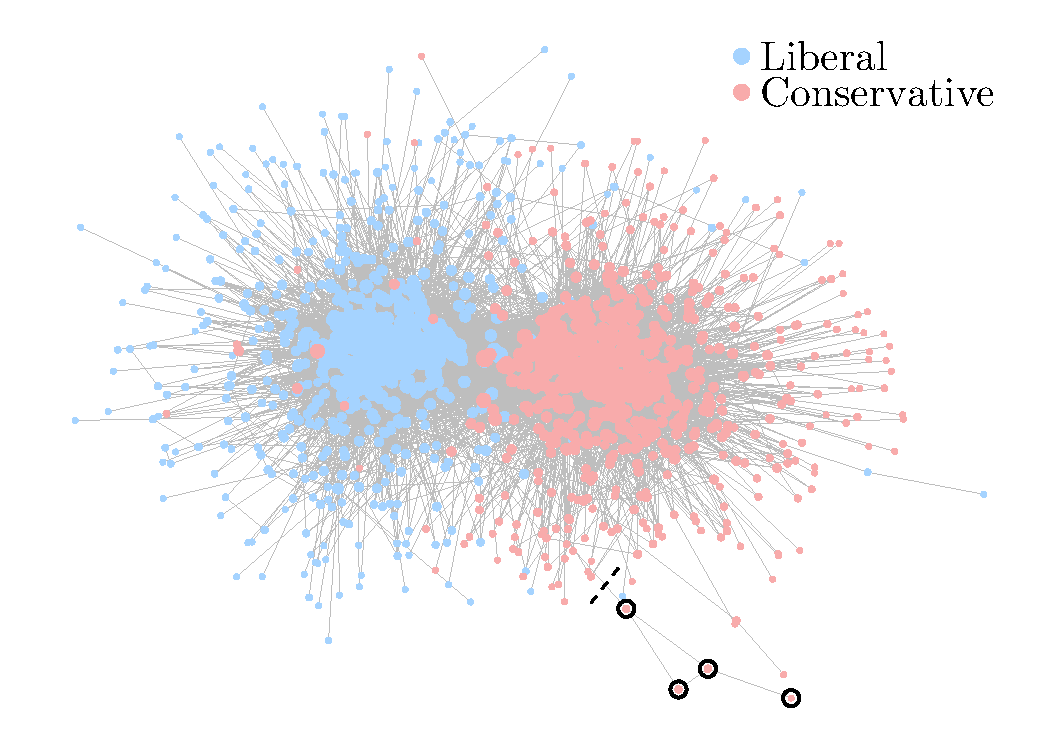
\includegraphics[scale=0.4,draft=false]{../../results/polblogs/polblogs_network.pdf}
		\caption{The US Political Blogs network}
		\label{fig:polblogs_network}
	\end{subfigure}
	\begin{subfigure}{.49\textwidth}
		\centering
		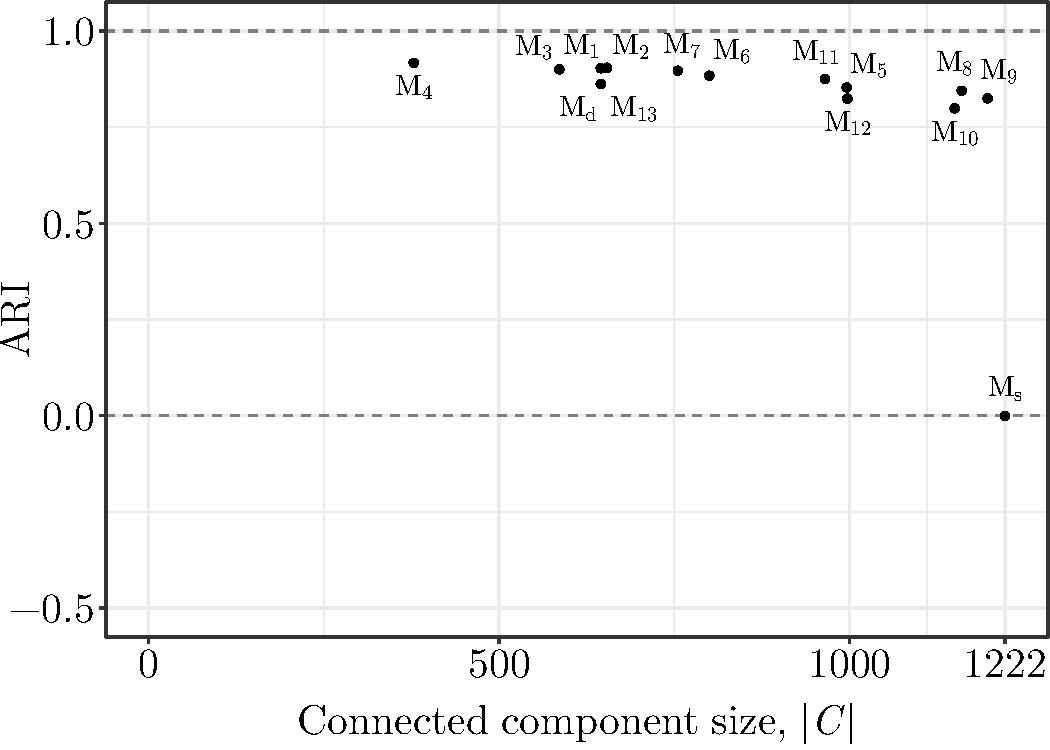
\includegraphics[scale=0.4,draft=false]{../../results/polblogs/polblogs_ari_conn.pdf}
		\caption{ARI against $|C|$ across motifs}
		\label{fig:polblogs_ariplot}
	\end{subfigure}
	\caption{Plots relating to the US Political Blogs network}
\end{figure}

Figure~\ref{fig:polblogs_embedding} shows the embedding given by eigenvectors 2 and 3 of the random-walk Laplacian of the MAM generated by motif $\ca{M}_{12}$. An instance of this motif in the network indicates the presence of a pair of mutually citing blogs with an incoming citation from a third (see Figure~\ref{fig:motif_definitions_directed}). Colourings are provided for Figure~\ref{fig:polblogs_embedding_truth} by the truth labels and for Figure~\ref{fig:polblogs_embedding_kmeans} by the $k$-means++ clustering of eigenvector 2. The clusterings are very similar, giving an ARI of $0.82$.


\vspace*{0.5cm}
\begin{figure}[H]
	\begin{subfigure}{.49\textwidth}
		\centering
		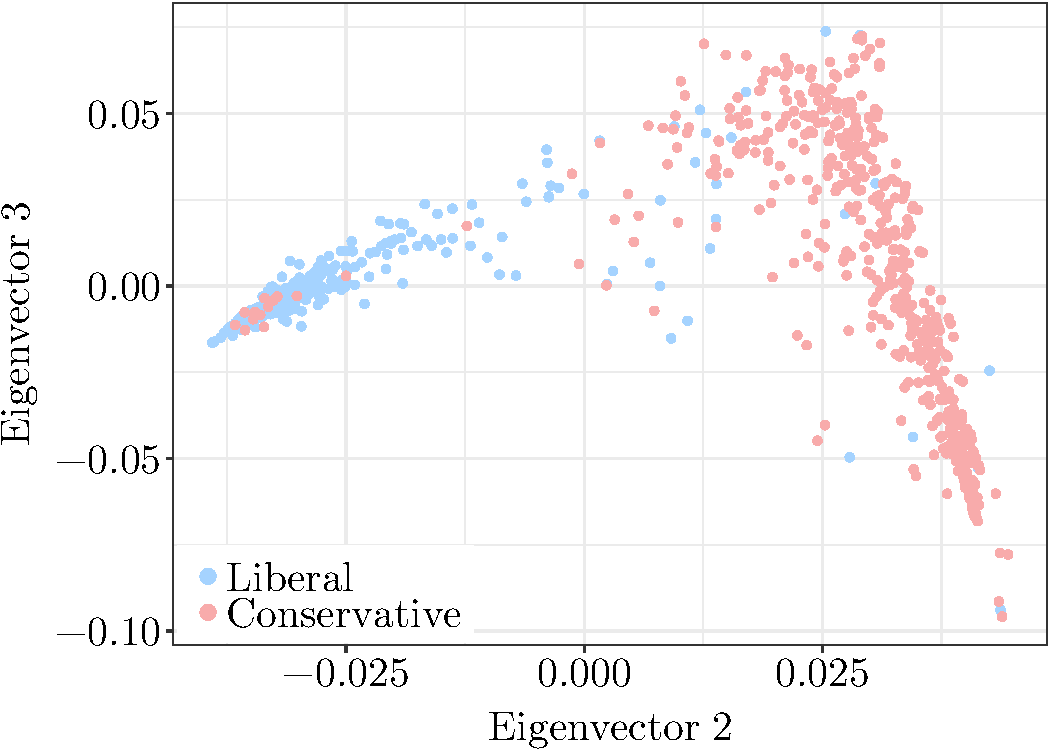
\includegraphics[scale=0.4,draft=false]{../../results/polblogs/polblogs_M12_truth.pdf}
		\caption{Colouring by truth label}
		\label{fig:polblogs_embedding_truth}
	\end{subfigure}
	\begin{subfigure}{.49\textwidth}
		\centering
		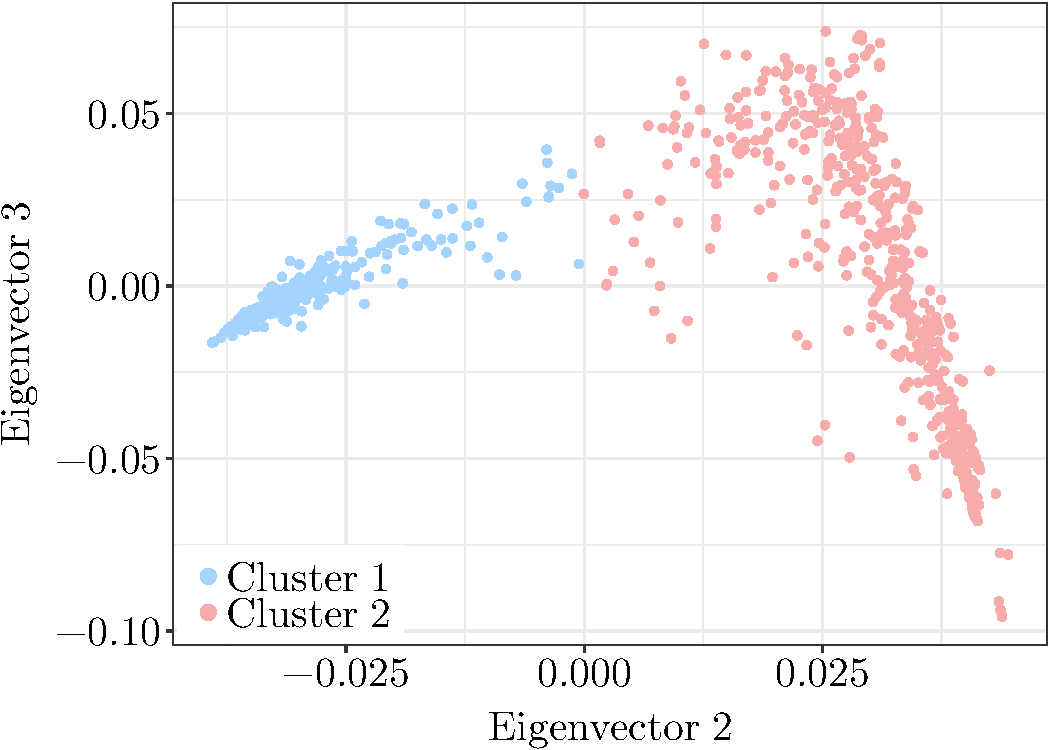
\includegraphics[scale=0.4,draft=false]{../../results/polblogs/polblogs_M12_clusts.pdf}
		\caption{Colouring by $k$-means++ cluster}
		\label{fig:polblogs_embedding_kmeans}
	\end{subfigure}
	\caption{Eigendecomposition embedding of the US Political Blogs network}
	\label{fig:polblogs_embedding}
\end{figure}










\pagebreak

\section{US Migration network} \label{sec:motif_migration}

The next data set is the US Migration network \cite{census2000}, consisting of data collected during the US Census in 2000. Vertices represent the 3075 counties in 49 contiguous states (excluding Alaska and Hawaii, and including the District of Columbia). The $721\,432$ weighted directed edges represent the number of people migrating from county to county, capped at $10 \, 000$ (the 99.9th percentile) to control large entries, as in \cite{DirectedClustImbCuts}.

We test the performance of Algorithm~\ref{alg:motifrwspectclust} with three selected motifs: $\ca{M}_\mathrm{s}$, $\ca{M}_6$ and $\ca{M}_9$ (see Figure~\ref{fig:motif_definitions_directed}).
$\ca{M}_\mathrm{s}$ gives the traditional spectral clustering method with na\"ive symmetrisation.
$\ca{M}_6$ represents a pair of counties exchanging migrants, with both also receiving migrants from a third.
$\ca{M}_9$ is a path of length two, allowing counties to be deemed similar if there is migration between them via another.

Firstly, we plot sweep profiles of the graph using the second eigenvector of the random-walk Laplacian of the MAM associated with each motif, in Figure~\ref{fig:migration_sweep}. Note that all three display clear minima, indicating that these motifs produce well-defined clusters. The two-part clusterings produced by eigenvector sweep are somewhat similar across the three motifs, with pairwise ARIs equal to $\textrm{ARI}(\ca{M}_\mathrm{s}, \ca{M}_6) = 0.67$, $\textrm{ARI}(\ca{M}_\mathrm{s}, \ca{M}_9) = 0.92$ and $\textrm{ARI}(\ca{M}_6, \ca{M}_9) = 0.73$.


\begin{figure}[H]
	\begin{subfigure}{.325\textwidth}
		\centering
		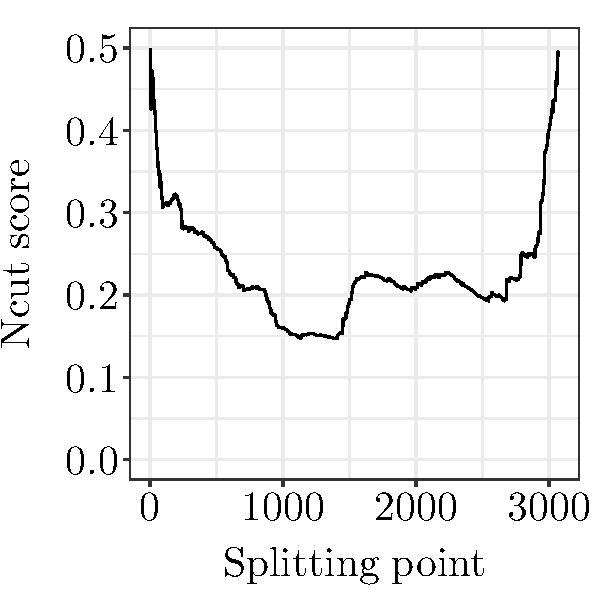
\includegraphics[scale=0.4,draft=false]{../../results/us_migration/us_migration_sweep_profile_Ms.pdf}
		\caption{$\ca{M}_\mathrm{s}$}
	\end{subfigure}
	\begin{subfigure}{.325\textwidth}
		\centering
		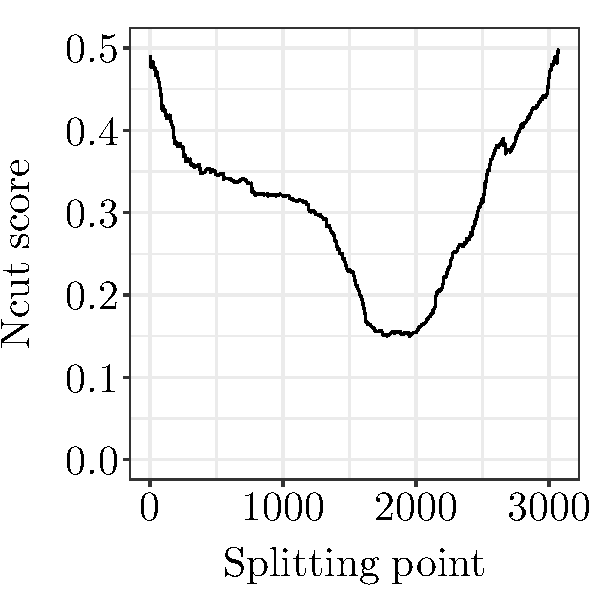
\includegraphics[scale=0.4,draft=false]{../../results/us_migration/us_migration_sweep_profile_M6.pdf}
		\caption{$\ca{M}_6$}
	\end{subfigure}
	\begin{subfigure}{.325\textwidth}
		\centering
		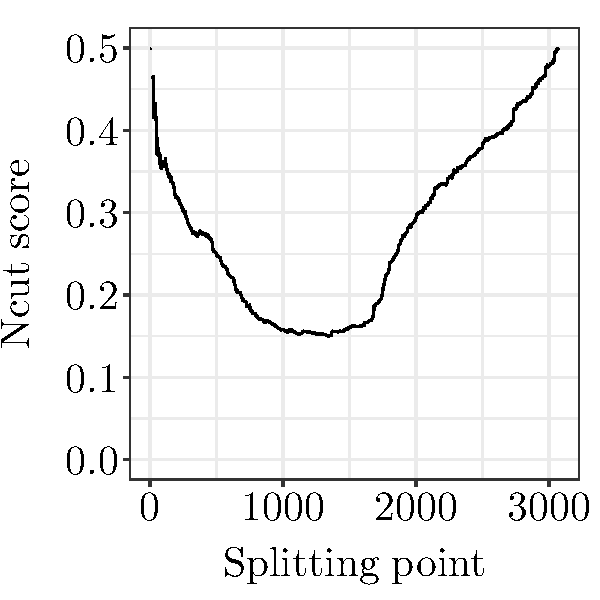
\includegraphics[scale=0.4,draft=false]{../../results/us_migration/us_migration_sweep_profile_M9.pdf}
		\caption{$\ca{M}_9$}
	\end{subfigure}
	\caption{Sweep profiles of the US Migration network}
	\label{fig:migration_sweep}
\end{figure}




Next, Figure~\ref{fig:us_migration} plots maps of the US, with counties coloured initially by the first six non-trivial eigenvectors $x_2, \ldots, x_7$ of the random-walk Laplacian of the associated MAM, and then by the clustering $C$ obtained by Algorithm~\ref{alg:motifrwspectclust} with $k=l=7$.

For the eigenvector colourings, note how the coloured regions often line up with state boundaries, indicating that many migrants stay within the same state.
It is also apparent that the motifs $\ca{M}_6$ and $\ca{M}_9$ produce `noisier' embeddings than traditional spectral clustering, due to their reliance on three-vertex motifs.
Eigenvector~2 approximately differentiates counties by longitude, although $\ca{M}_9$ achieves a clearer division between east and west, while $\ca{M}_\mathrm{s}$ and $\ca{M}_6$ colour California (CA, see Figure~\ref{fig:notes_us_map}) more similarly to the East Coast.
Eigenvector 3 tends to differentiate by latitude, though $\ca{M}_\mathrm{s}$ and $\ca{M}_6$ particularly isolate the states of North Dakota (ND), South Dakota (SD), Minnesota (MN), Wisconsin (WI) and Michigan (MI).
Further structure is visible across all three motifs for eigenvectors 4--7.

The clusterings $C$ partition the counties into $k=7$ regions, and there are some interesting differences between the motifs.
Since there is no ground-truth clustering, we record the Ncut score associated with each clustering.
It is apparent that motifs $\ca{M}_6$ and $\ca{M}_9$ give a similar partition, although with some differences:
$\ca{M}_6$ clusters the East Coast together with western Florida (FL) and the counties containing Los Angeles (CA), San Diego (CA), Las Vegas (NV), Phoenix (AZ), Tucson (AZ), Denver (CO), Chicago (IL) and Nashville (TN).
$\ca{M}_6$ favours a larger `central' region, which includes significant parts of Colorado (CO), Oklahoma (OK), Arkansas (AR) and Illinois (IL).
$\ca{M}_\mathrm{s}$ gives a somewhat different partition, with one of the clusters allocated to Michigan (MI) and Wisconsin (WI) rather than Mississippi (MS), Alabama (AL), Georgia (GA) and Tennessee (TN). As with the eigenvectors, the clustering is smoother for $\ca{M}_\mathrm{s}$ than for $\ca{M}_6$ and $\ca{M}_9$.





\pagebreak

\vspace*{-1cm}
\begin{figure}[H]
	\begin{table}[H]
		\centering
		\setlength{\tabcolsep}{0em}
		\begin{tabular}{ |c|c|c|c| }
			\expandableinput ../../results/us_migration/us_migration_table.txt
		\end{tabular}
	\end{table}
	\vspace*{-0.5cm}
	\caption{Motif-based colourings of the US Migration network}
	\label{fig:us_migration}
\end{figure}
